\documentclass[12pt,oneside,a4paper,english]{article}
\usepackage[T1]{fontenc}
\usepackage[latin2]{inputenc}
\usepackage[margin=2.25cm,headheight=26pt,includeheadfoot]{geometry}
\usepackage[english]{babel}
\usepackage{listings}
\usepackage{xcolor}
\usepackage{amssymb}
\usepackage{colortbl}
\usepackage{rotating}
\usepackage{bigstrut}
\usepackage{titlesec}
\usepackage{titling}
\usepackage[framed, numbered]{matlab-prettifier}
\usepackage{changepage}
\usepackage{amsmath}
\usepackage{hyperref}
\usepackage{enumitem}
\usepackage{graphicx}
\usepackage{fancyhdr}
\usepackage{lastpage}
\usepackage{caption}
\usepackage{tocloft}
\usepackage{setspace}
\usepackage{multirow}
\usepackage{titling}
\usepackage{float}
\usepackage{comment}
\usepackage{booktabs}
\usepackage{indentfirst}
\usepackage{lscape}
\usepackage{booktabs,caption}
\usepackage[flushleft]{threeparttable}
\usepackage[english]{nomencl}
\usepackage{xcolor}
\usepackage{lipsum}
\bibliographystyle{apalike}
\usepackage{url}
\usepackage{subcaption}
\usepackage{natbib}
\usepackage[nottoc]{tocbibind}


% --- set footer and header ---
\pagestyle{fancy}
\fancyhf{}

\setlength{\parindent}{2em}
\title{Bachelorthesis - Report} % to reference as \title, dont use \maketitle
\makeatletter\let\Title\@title\makeatother



\lstset{language=Matlab,
style=Matlab-editor,
basicstyle=\normalsize\mlttfamily,
numbers=left,
numberstyle={\scriptsize\color{black}},			% size of the numbers
numbersep=0.5cm											
}

\newlist{steps}{enumerate}{1}
\setlist[steps, 1]{leftmargin=1.5cm,label = Step \arabic*:}
\renewcommand{\headrulewidth}{1pt}
\renewcommand{\footrulewidth}{1pt}

%\lhead{\Title}
\rhead{\nouppercase{\rightmark}}
\lhead{\Title}
\rfoot{
\includegraphics[height=1.25cm]{Darmstadt.png}} % right header logo
\setlength\headheight{16pt}
\setlength{\footskip}{50pt}
\lhead{\Title} %rightH title
\cfoot{\thepage}
\captionsetup[table]{position=bottom}
% --- End of page settings ---



\begin{document}
\pagenumbering{roman} 

\begin{titlepage}
\begin{center}
\vspace{2cm}
%\textsc{ Danmarks Tekniske Universitet}\\[1.5cm]

\includegraphics[width=0.75\textwidth]{Darmstadt.png}~\\[1cm]
\vspace{1cm}

\vspace{2cm}

% Title
\hrule
\vspace{.5cm}
{ \huge \bfseries Data-driven modeling of self-ignition properties of the renewable fuel PODE (Polyoxymethylen Dimethyl ether) using methods of machine learning} % title of the report
\vspace{.5cm}

\hrule
\vspace{1.5cm}

\textsc{\textbf{Author}}\\
\vspace{.5cm}
\centering
% add your name here
Pascal Roth - 2541363\\
\vspace{1.5cm}

\textsc{\textbf{Advisers}}\\
\vspace{.5cm}
\centering
% add your name here
Philip Haspel, M. Sc.\\
Julian Bissantz, M. Sc. 
\vspace{1.5cm}

\centering \today % Dags dato
\end{center}
\end{titlepage}

\newpage
\doublespacing
%\addcontentsline{toc}{section}{Table of Contents}
\renewcommand{\baselinestretch}{1}\normalsize
\tableofcontents
\renewcommand{\baselinestretch}{1}\normalsize
%\singlespacing
\thispagestyle{fancy} % force page style

\pagenumbering{arabic} 
\fancyfoot[C]{Page \thepage\ of \pageref{EndOfText}}
\newpage

\section{Literature Research} %%%%%%%%%%%%%%%%%%%%%%%%%%%%%%%%%%%%%%%%%%%%%%%%%%%%%%%%%%%%%%%%%%%%%%%%%%%%%%%%%%%

\subsection{\cite{toulson2010}} %%%%%%%%%
\textbf{Modeling the Auto-Ignition of Oxygenated Fuels using Multistep Model }

\begin{itemize}
\item{for rapid compression machines}
\item{750-925K; 10-46 atm; 0.5 to $\lambda=1$}
\item{simulate the ignition of biofuels and their blends}

	\begin{itemize}
	\item{because: chemistry of biodiesel unknown; no kinematic mechanism available}
	\item{because: next year aim to optimize biofuels}
	\end{itemize}

\item{RCM:}

	\begin{itemize}
	\item{loss complicated fluid mechanics/ near Wall mixing}
	\item{heat test fuel as fast as possible (50\% compression 3ms) $\rightarrow$ less radicals}
	\end{itemize}
	
\item{important to model compression stroke $\rightarrow$ accurately predict ignition delay}
\item{Multistep-Model: only valid for one fuel $\rightarrow$ has to be changed with every small change}
\item{Model: 8 equations/ 7 species/ 26 constants}
\item{Heat Loss Model $\rightarrow$ do we have such data?}
\item{$V_{add}$ as an empirical parameter is used to account the effect of heat loss}
\item{CHEMKIN $\rightarrow$ instead we use Cantera}
\item{shock tubes more accurate as RCM $\rightarrow$ due to measurement of ignition delay }
\item{CHEMKIN high computational effort}	
\item{Model test}

	\begin{itemize}
	\item{increase the ignition delay that occurs with decreasing compressed pressure}
	\item{given temperature, decreased ignition delay that arises as the equivalence rate changes from 0.5 to $\lambda = 1$}
	\end{itemize}

\end{itemize}


\subsection{\cite{vandersickel2013}} %%%%%%%%
\textbf{Global Reaction mechanism for the auto-ignition of full boiling range gasoline and kerosene fuels}

\begin{itemize}
\item{predicting auto-ignition = pre-requisite for control/ optimize HCCI}
\item{model can be applied to any hydrocarbon fuel (with adjustment of parameters)}
\item{HCCI $\rightarrow$ low fuel consumption and low emissions}

	\begin{itemize}
	\item{depends from the fuel $\rightarrow$ fuel impact on engine design/ control strategy}
	\item{depends on operation conditions $\rightarrow$ initial charge conditions, engine load speed}
	\end{itemize}

\item{Model necessary to run multidimensional CFD}
\item{Why global reaction mechanism?}
	
	\begin{itemize}
	\item{only a limited number of species/ global quantities of interest}
	\item{cover a wide range of fuels and operating conditions}
	\item{provide reaction schemes for fuels for which no reaction scheme is available at the moment}
	\end{itemize}
	

\item{predicts important trace species and their evolution for homogeneous HCCI}
\item{model with 7 equations, pre-exponential factor $R_{3t}S_{3t}$ for each fuel separately make model applicable for every fuel} 
\item{use of 3 optimization function, 2 for the ignition delays of the first and second stage ignition, third for the pressure}

	\begin{itemize}
	\item{no realistic species profile}
	\item{because low and high temperatures are only coupled over temperature}
	\item{solution: forth objective function to ensure realistic rates}
	\end{itemize}

\item{leads to non unique solutions}
\item{perfectly homogeneous conditions $\rightarrow$ \textbf{add noise to NN to improve realistic conditions}}
\item{for major combustion products $CO, CO_2, H_2O$ qualitatively and quantitatively good comparison}
\item{intermediate species are grouped together or already added to the main species, reason why some graphs are too high}
\item{optimization over one more parameter $\rightarrow$ more effect}

	\begin{itemize}
	\item{Trade-Off: Accuracy $\leftrightarrow$ Computational Effort}
	\end{itemize}
	
\item{shock tube data reflects the purely chemical behavior is to be preferred over engine data}
\item{covers the two ignition behavior of full boiling range fuels $\rightarrow$ can show strong and weak NTU behavior} \\
\end{itemize} 


\subsection{\cite{sun2017}} %%%%%%%%%
\textbf{Speciation and the laminar burning velocities of $POMDME_3$ flames}

\begin{itemize}
\item{oxygenated alternative fuel $\rightarrow$ soot-reduction potential}
\item{26 species/ radicals, low pressure, $\lambda=$ 0.7 - 1.6, atm}
\item{laminar premixed flame}
\item{$POMDME_n$ with $n>1$ $\rightarrow$ directly applied for engines; high cetan number and large oxygen contents, but flow ability decreases}
\item{lower soot/PAH emissions $\leftrightarrow$ increase emissions of CO/ formaldehyde}
\item{parameters have been found over an analogy}
\item{under low-pressure premixed flames $\rightarrow$ fuel consumed through hydrogen abstraction}

	\begin{itemize}
	\item{could change with higher temperature and pressure in rapid compression engines} \\
	\end{itemize}

\end{itemize}


\subsection{\cite{He2018}} %%%%%%%
\textbf{A chemical kinetic mechanism for the low and intermediate temperature combustion of Polyoxymethylene Dimethyl ether}

\begin{itemize}
\item{Why $PODE_n$?}

	\begin{itemize}
	\item{CO alternating chain structure}
	\item{high cetan number}
	\item{high oxygen content $\rightarrow$ less soot precursors}
	\item{no bonds between carbon atoms $\rightarrow$ reduce particulate-matter (PM) emissions}
	\item{without PM emissions $\rightarrow$ higher rate of exhaust gas recirculation (EGR) possible $\rightarrow$ reduce $NO_x$ emissions}
	\item{finish trade off between soot and $NO_x$ emissions }
	\item{good ignitability $\rightarrow$ reduce CO and unburned carbon (HC)}
	\end{itemize}
	
\item{$PODE_n$ is non-toxic and miscible with diesel fuel in any desired ratio without changing the engine design $\rightarrow$ but engine optimization for it still possible}
\item{cost of production close to diesel (China $\leftrightarrow$ Germany??)}
\item{$PODE_3$ best suitable of its kind}

	\begin{itemize}
	\item{$PODE_1$ not suitable, cause ''gas lock effect'', low cetan number}
	\item{$PODE_2$ not suitable, flash point is too low to fulfill security}
	\item{$PODE_{n>5}$ not suitable, cannot handle low temperature}
	\end{itemize}
	
\item{mechanism based on assumption: reactions for $PODE_n$ similar to regular alkans}

	\begin{itemize}
	\item{difference: due to C-C bonds, no formation of alkans}
	\end{itemize}

\item{rate constant taken from $PODE_1$ and consumption between DME and DEE}
\item{thermodynamic properties: enthalpy, entropy, heat capacity}
\item{assuming adiabatic core region in RCM $\rightarrow$ homogeneous reactor model}

	\begin{itemize}
	\item{initial conditions: effective pressure and temperature, initial test gas composition}
	\end{itemize}

\item{HCCI engine $\rightarrow$ SAGE combustion model}
\item{no spray submodels used: distributed homogeneously in cylinder}
\item{automated grid size by looking at gradients}
\item{ignition delay = end of the compression and the maximum rate of pressure rise due to the ignition}
\item{lowest energy stable structure $\rightarrow$ spiral}
\item{negative temperature coefficient (NTC) effect is not evident in the combustion of $PODE_3$}
\item{current mechanism for $PODE_3$ consistently overestimated the total ignition delay time}

	\begin{itemize}
	\item{because of assumptions of ideal compression}
	\item{over 800K heat release of oxidation out stands} \\
	\end{itemize}

\end{itemize}

 
\subsection{\cite{Jacobs2019}} %%%%%%%%%%%
\textbf{An experimental and theoretical comparison of the novel e-fuel class oxymethylene ethers}

\begin{itemize}
\item{premixed OME under engine conditions}
\item{reduce soot, improves trade-off between $NO_x$ and PM}
\item{diesel-like properties more prominent $x=3-4$ (increased chain length)}

		\begin{itemize}
		\item{with $x>2$ higher cetane number than diesel}
		\end{itemize}

\item{Sun et al. $\rightarrow$ measured laminar burning velocities and intermediate species (low pressure) and preliminary kinetic mechanism for high temperature}
\item{He et al. $\rightarrow$ ignition delay times of $OME_3$ /oxygen/ nitrogen mixtures at low/ intermediate temperatures (highly dilated conditions at lean, stoichiometric and rich conditions) and mechanism}
\item{this study: auto-ignition behavior of neat $OME_x$}
\item{long chains lead to shorter ignition delay times (IDT)}
\item{$OME_x$ shows no NTC regime}
\item{$OME_1$ monotonic increase, $OME_{2,3}$ between 800 and 960K no change}
\item{$IDT_3$ of $OME_x$ don't correlate with derived cetane number (DCN)}
\item{$OME_1$ has an unfavorable combustion behavior}
\item{$OME_{2,3}$ higher reaction rate due to $\beta$-scission reaction on secondary carbon}
\item{models are not able to accurately predict these IDTs} \\
\end{itemize}


\subsection{\cite{Cai2019}} %%%%%%
\textbf{An experimental and theoretical comparison of the novel e-fuel class oxymethylene ethers}

\begin{itemize}
\item{e-fuels = synthetic, carbon neutral fuels from $H_2O$ and $CO_2$ by renewable electricity via catalytic conversion}
\item{this study: accurate chemical mechanism for the auto-ignition of $OME_{2-4}$}

	\begin{itemize}
	\item{mechanism with generation framework based on reaction classes and rates which uses $OME_1$ reaction rate constants and transfer then to $OME_{2-4}$; use $OME_1$ to guarantee chemical correctness}
	\end{itemize}

\item{graph theory: three dimensional molecule structures which show information about the precedence (H-Atoms and unpaired electrons) and their bonds (edges and verticals) $\rightarrow$ quantum chemistry calculations possible}

	\begin{itemize}
	\item{derived reactions and rate constants should be further improved}
	\end{itemize}

\item{optimization $\rightarrow$ reduce parameters by categorizing similar kinetic reactions}

	\begin{itemize}
	\item{optimizing for different fuels at the same time}
	\end{itemize}

\item{optimization $\rightarrow$ using the thermochemical values}
\item{development process only valid for large molecules} \\
\end{itemize}


\subsection{Additional Paper} %%%%%%%%%
\begin{itemize}
\item{\cite{Lin2019} - Development of a compact and robust Polyoxymethylene Dimethyl Ether 3 reaction mechanism for internal combustion engines}

	\begin{itemize}
	\item{develop a mechanism in 2 steps: firstly a $PODE_3$ sub mechanism and secondly a primary reference fuel (PRF) mechanism, the combined (based on the \cite{Ren2019} model development}
	\item{advantages}
	
		\begin{itemize}
		\item{compact and reliable mechanism $\rightarrow$ 61 species and 190 reactions)}
		\item{the NTC is successfully captured by paying attention to an important endothermic reaction}
		\end{itemize}
	
	\item{validated with ignition delay times, laminar flame speed and flame species concentrations}
	\item{compared with \cite{He2018}, who's mechanism is generated by a transfer from $POME_1$ to $POME_3$}	
	\end{itemize}

\item{\cite{Lv2019} - Development of a compact and robust Polyoxymethylene Dimethyl Ether 3 reaction mechanism for internal combustion engines}

	\begin{itemize}
	\item{n-heptane - n-butylbenzen - $PODE_n$-polycylic aromatic hydrocarbon (PAH) mechanism $\rightarrow$ modeling the behavior of a diesel-$POME_n$ mixture, prior mechanism only used n-heptane as representative substance of diesel, this study adds n-butylbenzen as representative substance of aromatic hydrocarbons}
	\item{detailed mechanism of $POME_n$ therefore simplified by methods of rate of production (ROP)}
	\item{ether as fuel with the highest efficiency for reducing soot emissions cause ester has direct $CO_2$ group and oxygen content of alcolhol too low, furthermore highest cetane number}
	\item{$PODE_n$ has low vapor pressure, high oxygen content and high cetane number $\rightarrow$ most promising ether fuel}
	\item{50$\%$ $PODE_{3-5}$ high temperature region in cylinder expands and flame-propagation speed increased and reduces all kinds of emissions}
	\item{simplified n-butylbenzene sub-mechanism was coupled to the n-heptane-PAH mechanism by decoupling method, and the simplified n-heptane-n-butylbenzene-PAH model was obtained via corresponding adjustment and optimization}
	\item{$PODE_3$ mechanism by simplifying the detailed mechanism by \cite{He2018} (DRGEP method removes insignificant species and reactions in an iterative manner, as soon as deviation between step too big, simplification stopped}
	\item{then simplified $PODE_3$ model included in n-heptane-n-butylbenzene-PAH base model which had to be optimized}
	\item{no fundamental experimental studies on used fuel mixed $\rightarrow$ only validated against experimental values of $PODE_3$ (base mechanism not changed)}
	\end{itemize}

\item{\cite{Huang2019} - Influence of n-butanol-diesel-PODE fuels coupled pilot injection strategy on combustion and emission characteristics of diesel engine}

	\begin{itemize}
	\item{experimental study with different $PODE_n$ concentrations}
	\end{itemize}


\item{\cite{Ren2019} - Development of a reduced polyoxymethylene dimethyl ethers (PODE) mechanism for engine applications}

	\begin{itemize}
	\item{complex $POM_n$ mechanism is simplified in an iterative manner and then combined with a reduced reference fuel mechanism $\rightarrow$ PRF-PODE mechanism}
	\item{base PRF-PAH mechanism:}
	
		\begin{itemize}
		\item{oxidation processes of n-heptane ($nC_7H_{16}$) and iso-octane ($iC_8H_{18}$) can represent the ignition and combustion characteristics of diesel and gasoline}
		\item{constructed by simplifying detailed LLNL gasoline surrogate mechanism}
		\end{itemize}
		
	\item{$PODE_3$ sub-mechanism}
	
		\begin{itemize}
		\item{mechanism of \cite{He2018} reduced in 4 steps: 1) DRGEP removes most unimportant reactions 2) isomers with similar thermodynamic properties are grouped 3) DRGEP again 4) sensitive analysis to remove everything DRGEP has missed}
		\item{leads to shorter ignition delay than the detailed mechanism since the reaction flow becomes more direct and effective}
		\item{ only carbonyl species containing CO bonds are produced in the oxidation process of PODE instead of alkenes due to the absence of CC bonds in the molecular structure of PODE}
		\end{itemize}
	
	\item{two mechanism are combined and duplicated reactions are removed from the $PODE_3$ sub-mechanism while the base mechanism is kept unchanged}
	\item{in addition a reduced $NO_x$ mechanism is incorporated}
	\end{itemize}

\end{itemize}
\newpage %%%%%%%%%%%%%%%%%%%%%%%%%%%%%%%%%%%%%%%%%%%%%%%%%%%%%%%%%%%%%%%%%%%%%%%%%%%%%%%%%%%%%%%%%%%%%%%%%%%%%%

\section{Coupling Chemical and Thermal Analyses of Reacting Systems}

\begin{itemize}
\item {chemical kinetics with fundamental conservation principles (mass and energy conservation)}
\item {hence calculation of system temperatures, various species concentrations as functions of time (an known reactants and products)}
\item {without mass diffusion}
\item {assumptions of all models: systems are perfectly mixed and homogeneous in composition (except form plug-flow reactor $\rightarrow$ ignores mixing and diffusion in flow direction)}
\end{itemize}

\begin{figure}[H]
\centering
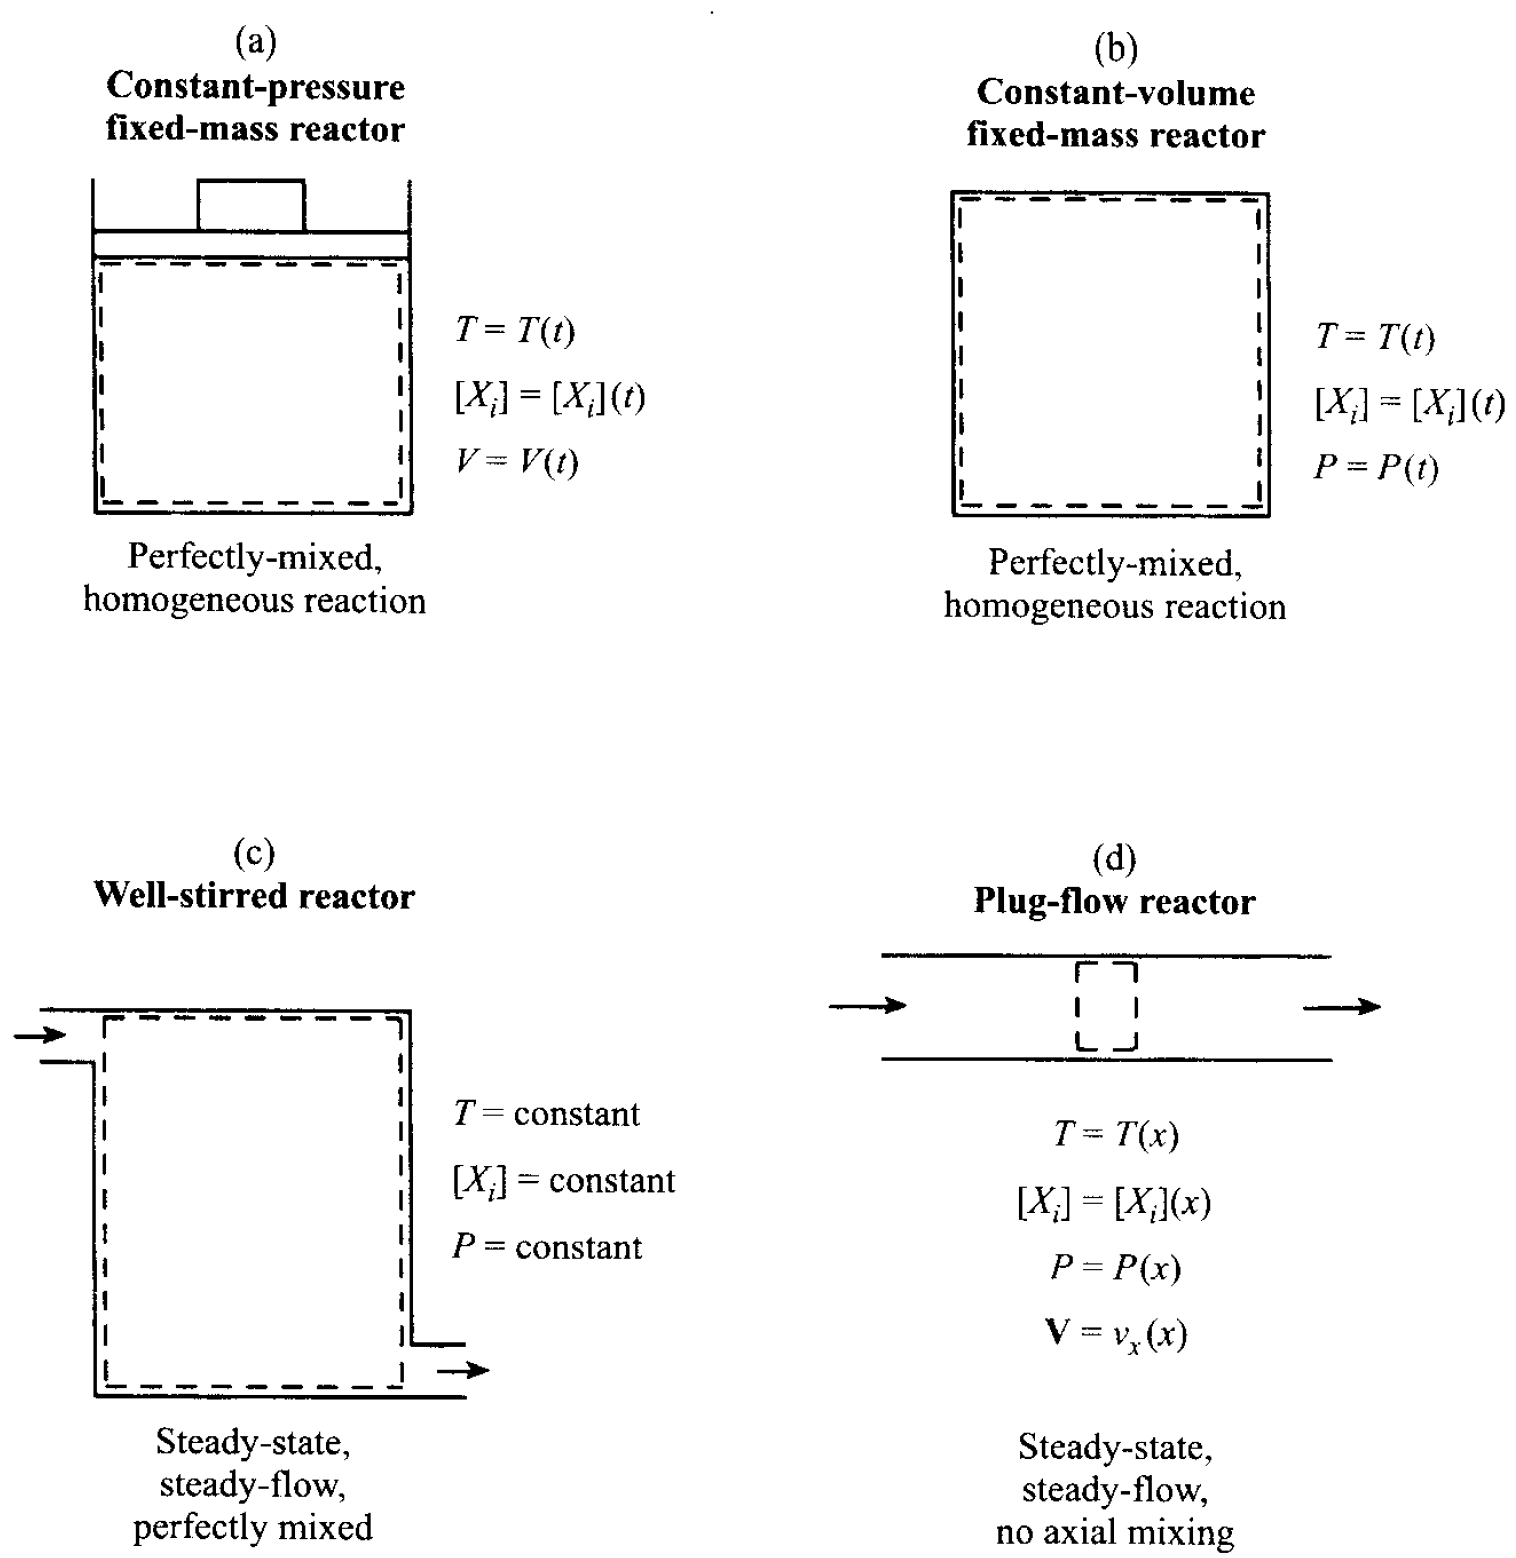
\includegraphics[width=0.5\textwidth]{models}
\caption{Four different reactor models (\cite{turns2012introduction})}
\label{fig:reactors}
\end{figure}


\subsection{Constant-pressure and fixed-mass reactor} %%%%%%

\begin{itemize}
\item {react at each and every location within the gas volume at the same rate}

	\begin{itemize}
	\item {no temperature or composition gradients within the mixture}
	\item {temperature and set of species enough to describe system}
	\end{itemize}

\item {exothermic reaction $\rightarrow$ temperature/ volume increase (and heat transfer through walls)}
\item {first order differential equations as initial-value problem}
\item {starting with the first law of thermodynamics and assuming that only $P-dv$ work leads to}

\begin{equation}
\frac{\dot{Q}}{m}=\frac{dh}{dt}
\end{equation}

\item{connection to chemical composition over enthalpy and further to the temperature which relates to the specific heat of species $i$, therefore assuming ideal-gas behavior}

\begin{align}
\frac{dh}{dt} &= \frac{1}{m}\left[ \sum_i (\bar{h}_i \frac{dN_i}{dt}) + \sum_i (N_i \frac{d \bar{h}_i }{dt}) \right] \\
 &= \frac{1}{m}\left[ \sum_i (\bar{h}_i \frac{dN_i}{dt}) + \sum_i (N_i \bar{c}_{p,i} \frac{dT}{dt}) \right] 
 \end{align}
 
 \item{the chemical composition can be further linked to the molar concentration $[X_i]$ and the mass-action expression $\dot{\omega}$ over the expression: $\frac{dN_i}{dt}=V \dot{\omega_i}$}
 \item {species molar concentrations $[X_i]$ change with time as a result of both chemical reactions and changing volume
 
 \begin{equation}
 \frac{d[X_i]}{dt}=\dot{\omega}_i - [X_i] \frac{1}{V} \frac{dV}{dt}
 \end{equation}
 
 where first time is for the chemical production and the second for the changing volume}
 \item{This leads to the two main equations to describe the reactor:}
 
 \begin{align}
 \frac{dT}{dt}=f([X_i],T) &= \frac{\frac{\dot{Q}}{V}-\sum_i (\bar{h}_i \dot{\omega}_i}{\sum_i ([X_i] \bar{c}_{p,i}} \\
 \frac{d[X_i]}{dt}=f([X_i],T) &= \dot{\omega}_i - [X_i] \left[ \frac{\sum \dot{\omega}_i}{\sum_j [X_j]} + \frac{1}{T} \frac{dT}{dt} \right]
 \end{align}
 
\end{itemize}


\subsection{Constant-volume, fixed-mass reactor} %%%%%%%%

\begin{itemize}
\item{similar to the reactor with constant pressure, but due to constant volume, no work $\rightarrow$ first law of thermodynamics:}

\begin{equation}
\frac{du}{dt}=\frac{\dot{Q}}{m}
\end{equation}

\item{in this way specific internal energy $u$ same role as prior specific enthalpy $h$, this leads to the characteristic equations which further include the time-rate-of-change of the pressure wit the definition of pressure: $P = \sum_i [X_i] R_u T$}

\begin{align}
 \frac{dT}{dt}=f([X_i],T) &= \frac{\frac{\dot{Q}}{V}-\sum_i (\bar{u}_i \dot{\omega}_i}{\sum_i ([X_i] \bar{c}_{v,i}} \\
 \frac{d[X_i]}{dt}=f([X_i],T) &= \dot{\omega}_i \\
 \frac{dP}{dt}=f([X_i],T) &= R_u T \sum_i \dot{\omega}_i + R_u \sum_i [X_i] \frac{dT}{dt}
 \end{align}
 
 \end{itemize}
 
 
\subsection {Well-stirred reactor} %%%%%%

\begin{itemize}
\item{perfect mixing due to high velocity}
\item{was used to obtain values for global reaction parameters}

\begin{figure}[H]
\centering
\includegraphics[width=0.5\textwidth]{Well_Stirred_reactor}
\caption{Schematic of a well stirred reactor (\cite{turns2012introduction}}
\label{fig:well-stirred-reactor}
\end{figure}

\item{for mass conservation with the generation term as a source or sink of the species:}

\begin{align*}
\frac{dm_{i,cv}}{dt} &= \dot{m}_i^m V + \dot{m}_{in} - \dot{m}_{out} \\
\text{Mass rate} &= \text{generated mass} + \text{Mass flow into} - \text{Mass flow out}
\end{align*}

\item {assumed to operate in a steady state mode there are no time dependencies! therefore the mass generation is only linked to $\dot{m}_i^{'''}=\dot{\omega}_i MW_i$ and the mass flow rates to $\dot{m}_i=\dot{m}Y_i$}
\item{with the steady flow conservation of energy equation 

\begin{equation}
\dot{Q}=\dot{m} \left( \sum_{i=1}^N Y_{i,out}h_i(T) - \sum_{i=1}^N Y_{i,in} h_i (T_{in}) \right)
\end{equation}

all variables can be calculated as a set of coupled non-linear equations}

\end{itemize}


\subsection {Plug-flow reactor} %%%%%%%
\begin{itemize}
\item{Assumptions}

	\begin{itemize}
	\item{steady state, steady flow $\rightarrow$ no time dependencies}
	\item{no mixing in axial direction $\rightarrow$ turbulent mass diffusion negligible in flow direction}
	\item{one-dimensional flow $\rightarrow$ single velocity, temperature, composition enough to characterize the flow at any cross section}
	\item{ideal friction-less flow}
	\item{ideal gas behavior}
	\end{itemize}

\item{can be implemented as any particular one-dimensional geometry}
\item{reactor flow properties as functions of distance x}
\item{with mass, momentum, energy and species conservation generate solution}
\item{characteristic equations are $\frac{d\rho}{dx}$, $\frac{dT}{dx}$ and $\frac{dY_i}{dx}$, which are shown at page 204}

\end{itemize}

\subsection {Model Comparison} %%%%%%%%%

\begin{center}
 \begin{tabular}{|p{0.25\textwidth} | p{0.25\textwidth} | p{0.25\textwidth} | p{0.25\textwidth}|}
 \hline
Constant pressure; fixed mass & Constant volume; fixed mass & Well Stirred & Plug-flow \\ [0.5ex] 
 \hline\hline
time dependencies  & time dependencies & steady-state & steady-state \\ 
 \hline
 mass constant & mass constant & mass flow constant & mass flow constant \\
 \hline
 no temperature or composition gradients inside reactor & no temperature or composition gradients inside reactor & completely homogeneous inside reactor in geometric and time manners & geometric dependencies \\
 \hline
 volume changing work & no work done & no work done & no work done \\
 \hline
perfectly mixed & perfectly mixed & perfectly mixed & assumption of no mixing in axial direction \\ [1ex] 
 \hline
\end{tabular}
\end{center}

\newpage %%%%%%%%%%%%%%%%%%%%%%%%%%%%%%%%%%%%%%%%%%%%%%%%%%%%%%%%%%%%%%%%%%%%%%%%%%%%%%%%%%%%%%%%

\section{Implementation of Homogeneous reactor}
In this project the constant-volume and fixed-mass reactor will be used. This is due to the fact that in the moment of combustion the volume can be seen as nearly constant while the pressure arises. In the next step the piston would be moved due to the pressure increase so that in this case work is done and the constant-pressure and fixed-mass model would be used. 

\subsection{Optimization} %%%%%%%%%%%%
Source: \cite{vandersickel2013}

\begin{itemize}
\item{purpose: simulation data should match experimental data}
\item{parameters to be optimized: Arrhenius Eq. (pre-exponential factor $A_i$, activation energy $E_I$, rate constant $k_i$), pressure correction terms, exponents of the fuel and third body concentration}
\item{used algorithm: multi-objective genetic algorithm $\rightarrow$ error of each optimization function can be controlled separately}
\item{make sure realistic parameters $\rightarrow$ parameters constraint to lie between predefined boundaries}
\item{objective functions for ignition delay:

\begin{align}
f_{LT} &= \frac{1}{N_{LT}} \sum_{i=1}^{N_{LT}} |\tau_{1i}^{exp}-\tau_{1i}^{sim}| \\
f_{HT} &= \frac{1}{N} \sum_{i=1}^{N} |\tau_{2i}^{exp}-\tau_{2i}^{sim}|
\end{align}

with:}

	\begin{itemize}
	\item{$\tau^{exp}$ as the experimental ignition delay and $\tau^{sim}$ as the simulation ignition delay}
	\item{LT for low temperature and HT for high temperature}
	\item{N is the number of initial conditions}
	\end{itemize}

\item{first stage ignition = low temperature; defined as time till first local maximum in heat release profile}
\item{main stage ignition = high temperature; defined as time till global maximum in heat release profile}
\item{for evolution of heat release and species profiles, implementation of two additional optimization criteria}
\item{the third objective function concerns the pressure and says that it has to match at the end of the cool flame with the pressure of the detailed reaction mechanism (end of combustion nearly no difference, end of cool flame around 15\%)}

\begin{equation}
f_{p_{LT}} = \frac{1}{N_{LT}} \sum_{i=1}^{N_{LT}} \frac{|p_{1i}^{det}-p_{1i}^{sim}|}{|p_{1i}^{det}|}
\end{equation}

\item{do not necessary yield to realistic species profiles, because intermediate and high temperatures schemes in global reaction mechanism are directly coupled over temperature $\rightarrow$ forth objective function to ensure a correct profile of a stable intermediate species, in case of \cite{vandersickel2013} $I_2$ of the seventh equation of the presented global reaction mechanism}

\begin{equation}
f_{max_{R7}} = \frac{1}{N} \sum_{i=1}^{N} |t_{max_{R7i}}^{sim}-\tau_{2i}^{sim}|
\end{equation}

	\begin{itemize}
	\item{here $t_{max_{R7i}}^{sim}$ is the time when the maximum of the reaction rate of the intermediate species}
	\end{itemize}
	
\item{trade-off between the objective function $\rightarrow$ not unique solution, chose depending to importance of different objective functions} \\
\end{itemize}


\subsection{Two-staged auto-ignition} %%%%%%%%%%%%
\begin{itemize}
\item{auto ignition behavior partly depends on the octane number, with a low-octane number the two-staged behavior is clearly visible while with higher octane number as in most gasoline fuels the ignition should not be active under low temperature conditions, resulting in a single-stage behavior (\cite{Chung2015})}
\item{first ignition stage $\rightarrow$ low temperature\\
Internal isomerization is initialized by the abstraction of H-atoms and leads to formation of radicals which are exchanged internally. The number of radicals increases which includes an acceleration of the reaction rates and initializes an exothermic cycle $\rightarrow$ cool flame heat release. }
\item{Negative Temperature coefficient\\
With the rise of the temperature the reactions changes for example explained in \cite{vandersickel2013} where the oxygen addition to the alkyl radical becomes important. This change is equivalent to a termination step because the new radicals recombine to stable intermediates like $H_2O$ or $O_2$. Which reduces the overall reaction rate and hence causes NTC area}
\item{second ignition stage $\rightarrow$ high temperature\\
During NTC the temperature only rises slowly until reaction of $H_2O_2$ becomes important (>1000K), terminating the NTC regime and initiating a branched thermal explosion. Heat release is dominated by oxidation of the intermediates $CH_2O$ to $CO$ and successive oxidation of $CO$ to $CO_2$. } 
\item{ignition times are defined with the heat release curve: first stage ignition time = time till first local maximum, main ignition delay time = global heat release rate maximum}\\
\end{itemize}

\begin{figure}[H]
\centering
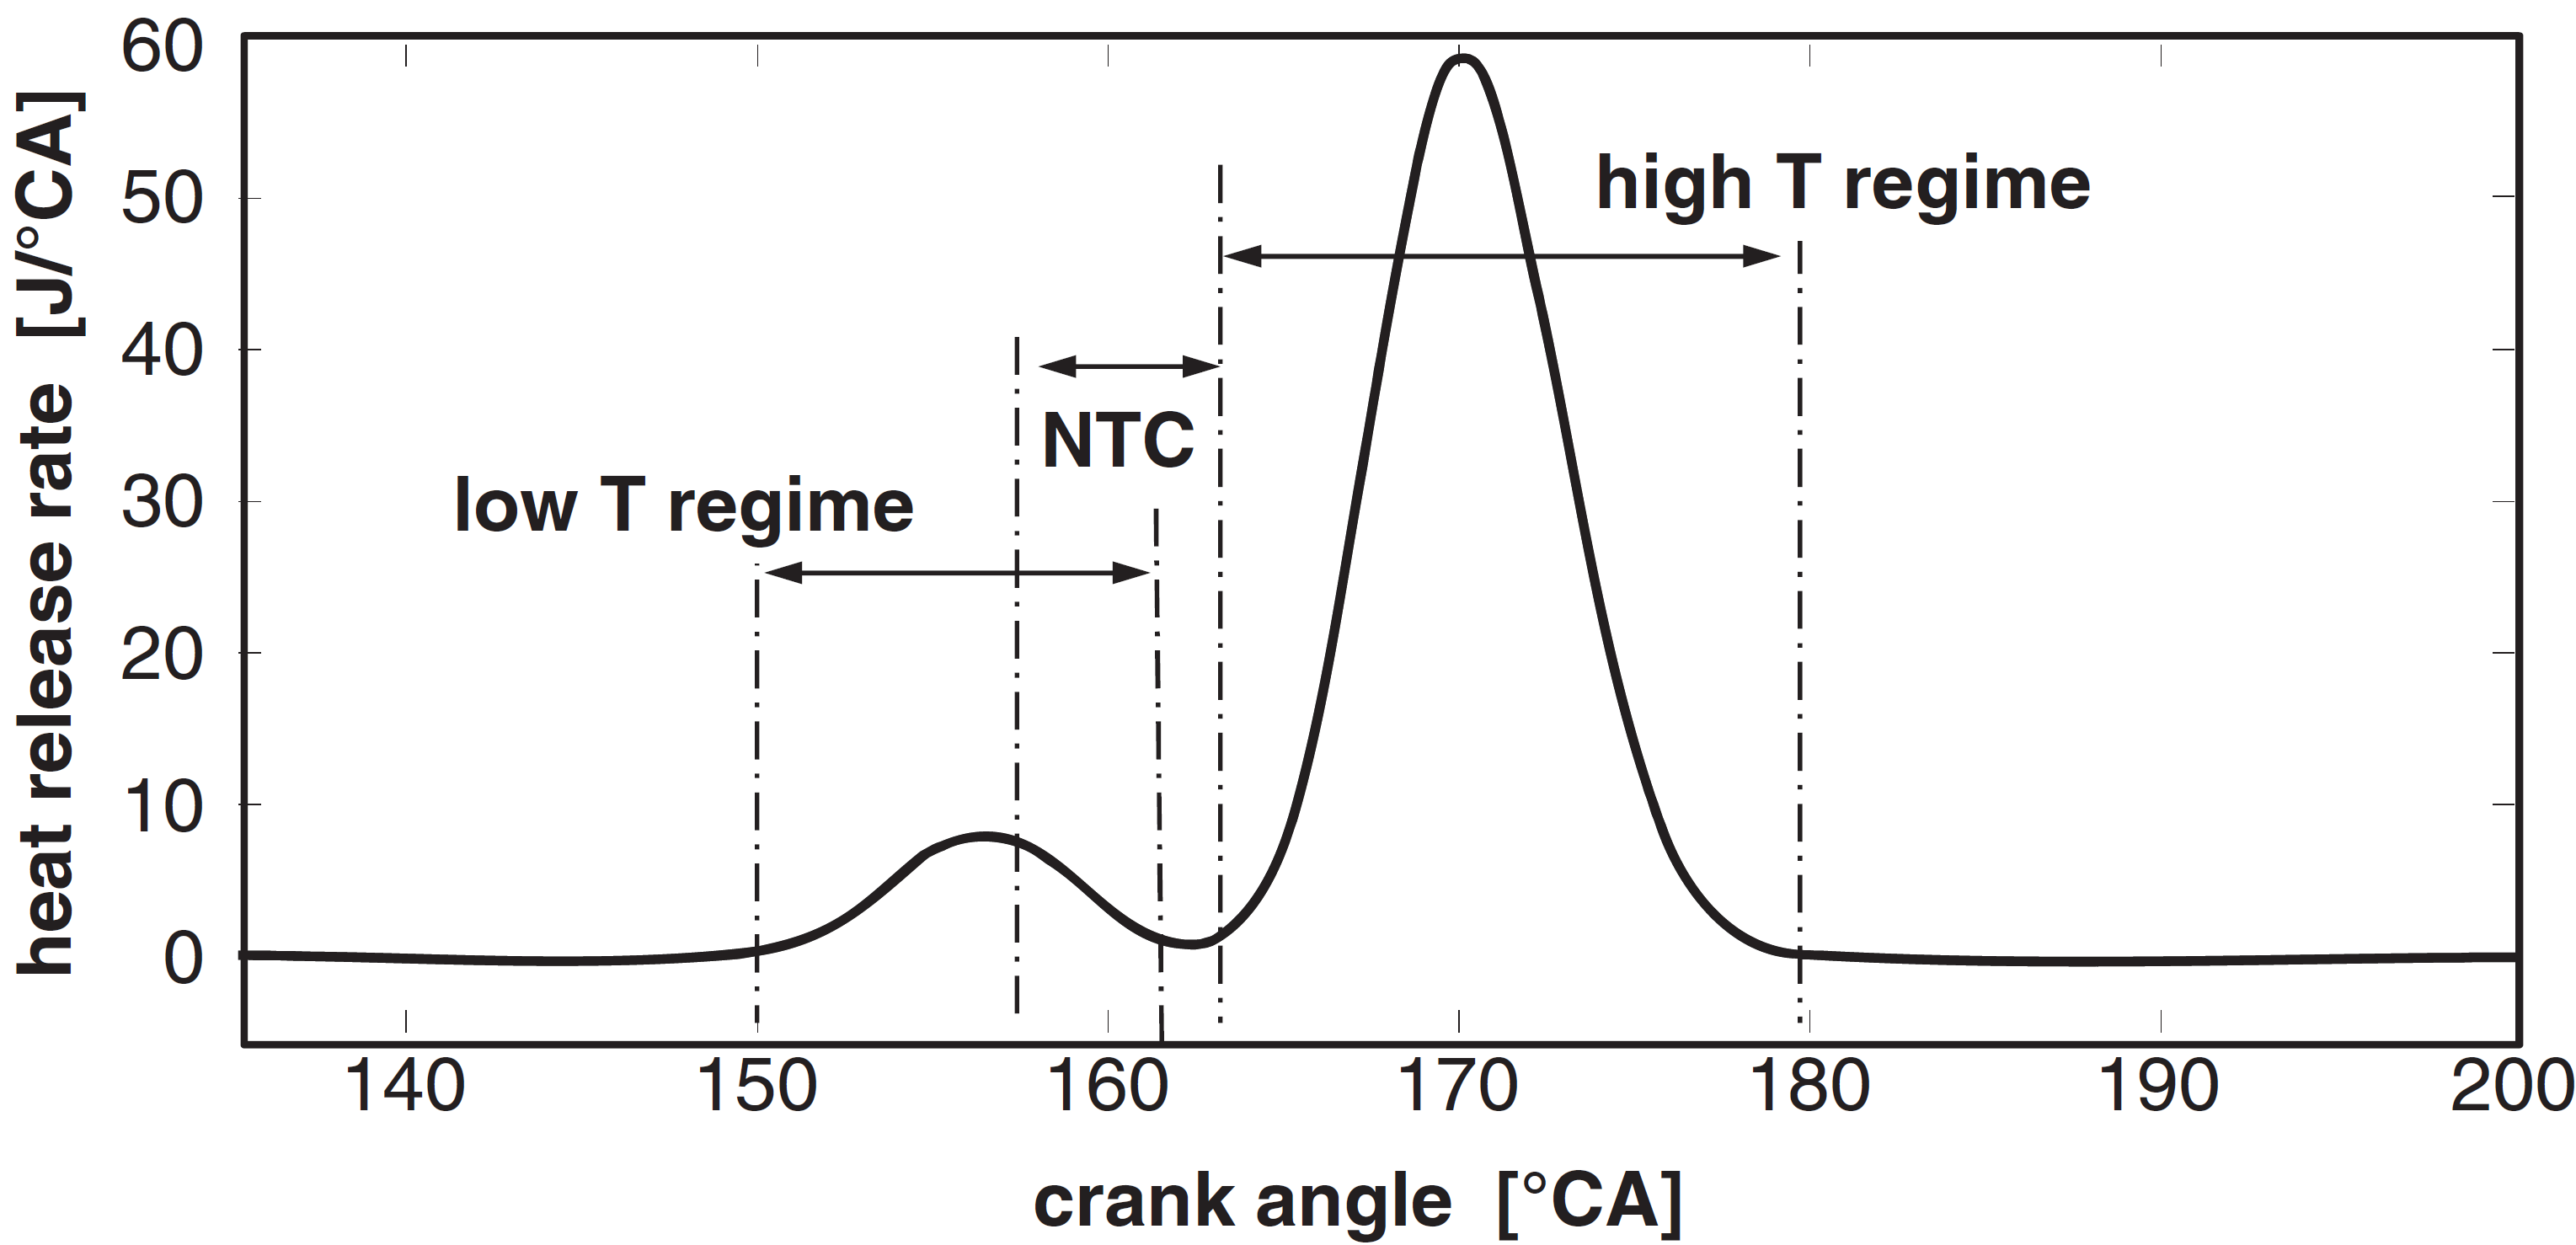
\includegraphics[width=0.5\textwidth]{two-stage-ignition}
\caption{Heat release profile for the two-stage ignition of teh HCCI combustion(\cite{vandersickel2013})}
\label{fig:two-stage-ignition}
\end{figure}


\subsection{Heat Release} %%%%%%%%%%%%
\label{heat_release}
\begin{itemize}
\item{assumption of an adiabatic reactor $\rightarrow$ no heat loss}
\item{but heat release inside the reactor $\rightarrow$ rise in temperature and pressure}
\item{cool flame heat release can count up to 15-20\% of heat release}

	\begin{itemize}
	\item{responsible for cool heat release reaction of $OH$-radicals with fuel and $O_2$ to $H_2O$ and $CO$}
	\end{itemize}
	
\item{heat release during the main ignition:}

	\begin{itemize}
	\item{first stage of main ignition: temperature enough to split up $H_2O_2$ to $2OH$ which results in an increase of the cool flame reaction}
	\item{as temperature rises high temperature scheme takes over}
	\item{mainly heat release through two reactions: $F+O_2 \rightarrow H_2O + CO$ and $CO + O_2 \leftrightarrow CO_2$ where the second reaction is dominant}
	\end{itemize}
	
\item{The first local maximum corresponds to the first stage ignition and the global maximum to the main ignition delay}
	
\end{itemize}


\subsection{Model parameters} %%%%%%%%%%%%%
\begin{itemize}
%\item{begin of ignition defined as the peak in the profile of OH species during combustion}
%\item{no intermediate species and no radicals to measure $\rightarrow$ will be done by NN}
\item{starting conditions:}

	\begin{itemize}
	\item{Air/ Fuel: $\theta$, $O_2:N_2$}
	\item{$T_{start}$ and $p_{start}$}
	\end{itemize}

\item{parameters, which value has to be captured at any point}

	\begin{itemize}
	\item{educts: $POME_n$; $O_2$}
	\item{products: $CO$, $CO_2$, $H_2O$}
	\item{intermediates: $OH$, $H_2O_2$}
	\item{Temperature and pressure}
	\item{heat release}
	\end{itemize}

\item{calculation of species while reactions take place}
	
	\begin{itemize}
	\item{mechanism only contains the reactions and their parameters}
	\item{\textbf{specific enthalpies} of all species depending on the temperature can be calculated with 
	
	\begin{equation}
	h_k = \Delta_{f,k}^{ref} + \int_{T_{ref}}^T c_{pk}dT
	\end{equation}
	
	where $h_k$ as the specific enthalpy of each species  and $c_{pk}$ as the species specific heat capacity depending the current and reference temperature ($\rightarrow$ use tabulated chemistry for specific heat capacities or directly for the enthalpy)}
	
	\item{\textbf{reaction enthalpy} can be calculated using the specific enthalpies of the reaction (possible that for the exact temperature linear interpolation has to be used, since not every value is listened in the table)
	
	\begin{equation}
	\Delta_{R,h} = \Delta \bar{h}_{products} - \Delta \bar{h}_{educts} 
	\end{equation}}
	
	\item{\textbf{concentration} at the time $t$ of each species has to be calculated next by using: 
	
	\begin{equation}
	C_{k,t} = Y_{k,t} * \frac{\rho_t}{\bar{M}_{k,t}}
	\end{equation}
	
	By making the assumption of an ideal gas $\rho$ can be replaced in the following way
	
	\begin{equation}
	C_{k,t} = Y_{k,t} * \frac{p_t*\frac{T_t}{\bar{R}*\bar{M}_{mean,t}}}{\bar{M}_{k,t}}
	\end{equation}}
	
	\item{the \textbf{rate constant} can be calculated with the Arrhenius Equation, therefore the pre-exponential factor $A$, the activation temperature $T_a$ of the reaction and the fitting rate constant $b$ has to be taken out of the chemistry tables:
	
	\begin{equation}
	k_{k,t} = A*T_t^b* exp(-\frac{T_a}{T_t})
	\end{equation}}
	
	\item{using the rate constant, the concentrations and the order of the reactions, the \textbf{reaction speed} can be calculated
	
	\begin{equation}
	r_{k,t} = k_{k,t}* \prod C_{x,t}^n 
	\end{equation}}
	
	\item{after having the reaction speed the mole factions of the time $t+1$ can be computed (using explicit Euler), for the Neural Net only the above listened must be saved}
	
	\item{sum of all reaction enthalpies multiplied with the mole fractions results in the heat release at a certain time}
	
		\begin{itemize}
		\item{The first local maximum corresponds to the first stage ignition and the global maximum to the main ignition}
		\end{itemize}
		
	\end{itemize}
	
\end{itemize}


\label{EndOfText}

\newpage %%%%%%%%%%%%%%%%%%%%%%%%%%%%%%%%%%%%%%%%%%%%%%%%%%%%%%%%%%%%%%%%%%%%%%%%%%%%%%%%%%%%%%%%

\bibliography{sample}


\pagenumbering{Roman} 

\thispagestyle{fancy}

\label{endOfDoc}
\fancyfoot[C]{Page \thepage\ of \pageref{endOfDoc}}
\end{document}